% !TeX root = ../report.tex

\section{Deep Learning} \label{sec:deep}
In this section, an overview of the model used in the "deep learning" attempt at solving task 1 and 5 will be presented. The model seeks to solve two subtasks in one go as a multitask learning problem. The subtasks are: regression (task 1 in section \ref{sec:task}) and classification (task 5 in section \ref{sec:task}). For task 1 the model also predicts independently of the general emotion felt, i.e. tweets for joy, anger etc. get a 0-to-1 score using the same model. \\
The multitask model itself a hard parameter sharing model, meaning the weights of the model is shared between the main and auxiliary task being solved, and the model itself is built in Keras, the Python based neural network wrapper for Tensorflow. 

\subsection{Model overview}

\subsubsection{Preprocessing of text and textual representation} \label{sec:preprop}
For the textual preprocessing, all tweets are read in and converted using a mapping from a word to an integer. This ensures that similar words get mapped to the same key and also enables an enforcing on the maximum amount of words to be used. Train data is treated differently than development and test data, in that every unique word read in train data gets converted to the word vector associated with the word. If an unknown word gets read in the development or test data its numerical value gets replaced by an "unknown" placeholder. One way of countering this is to use pretrained word embeddings. This does not constitute as having read and adapted to the test set, since one could envision having a pretrained word embedding for every word in the entire language. Furthermore, user mentions and numbers get mapped to a placeholder value instead of reading in their actual values.\\
The embedding weights used in the model are retrieved from a large set of pretrained embeddings which have been trained on Twitter data ($\sim$400 million tweets). The model used is created by the authors of \cite{godin}. The words in the dataset for the task at hand are then looked up in the pretrained embeddings. If these are not present a zero vector is used instead, which will then be trained from the ground up by the model.\\
Since the model used both word and character representations, the characters were read in separately, although the same basic principle was followed. Every character had a integer mapped to them and this integer would then map to a high dimensional vector with weights that could then be optimized by the network. No pretrained embeddings were used for the characters and so they had to be trained from the ground up, every time.

\subsubsection{Augmentation of data} \label{sec:augm}
The first iteration of the data augmentation consisted of reading in all the data for task 1 and 5 as described in section \ref{sec:preprop}. Since the tweets had different formats of truth labels, one was a singular value (regression) and one was a multi-label list (classification), reading in the labels had to be augmented. Since the tweets were reused in the two tasks, some of the regression tweets could be augmented with their respective classification label, although, if no classification label was present the truth labels were set to -1, which would then act as a mask. Since there were more regression tweets than classification, the augmentation was done this way around.\\
All the tweet representations were padded differently based on whether or not the tweet was being read as a word representation or character representation, and tweets longer than the specified padding values were cut down to size. 

\subsubsection{Word input model}
The word input to the model are 60  $\cdot$ 400 dimensional vectors that have been passed through the preprocessing and augmentation specified in section \ref{sec:preprop} and \ref{sec:augm}. These vectors are then passed into two 250-dimensional, bidirectional GRUs which traverse the tweet front to back and vice versa, and the outputs of the two GRU layers are then concatenated. This output is then batch normalized and a dropout is applied. This output of the word submodel is then concatenated later with the character submodel\\
\begin{figure}[H]
	\centering
		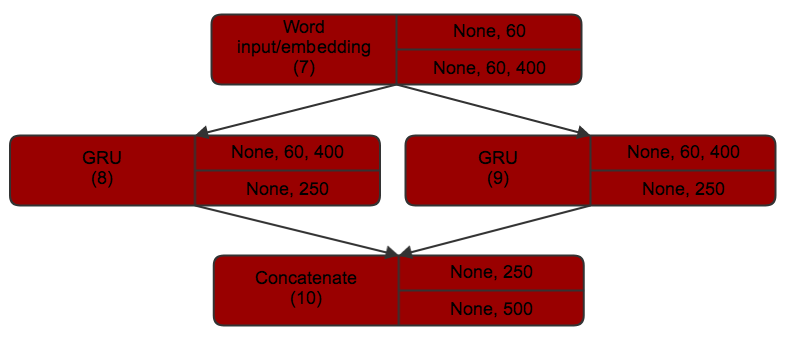
\includegraphics[scale=0.25]{pictures/word_model.png}
		\caption{The word input part of the full model}
		\label{fig:wordmodel}
\end{figure}
\subsubsection{Character input model}
The character input to the model are 256 $\cdot$ 400 dimensional vectors that have been through the same preprocessing and augmentation as the word inputs. These vectors then furthermore get passed into a residual neural network which works as a loop of batch normalizations, dropout applications and 1-dimension convolutions. Each loop ends with an layer-addition of the previous loop layer with the current loop layer and then a max pooling. These vectors are then passed into two GRU layers similar to the word input which are then concatenated and passed along to be connected with the word input part.
\begin{figure}[H]
	\centering
		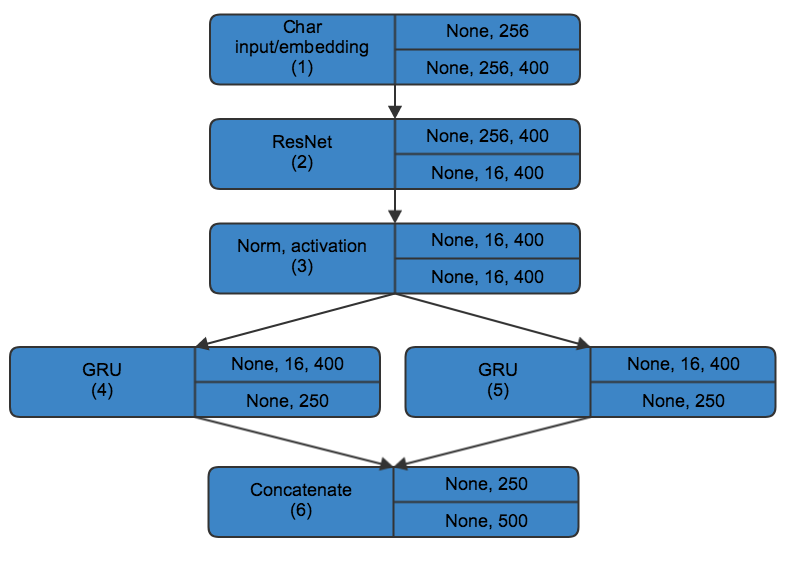
\includegraphics[scale=0.25]{pictures/char_model.png}
		\caption{The character input part of the full model}
		\label{fig:charmodel}
\end{figure}
\begin{figure}[H]
    \centering
        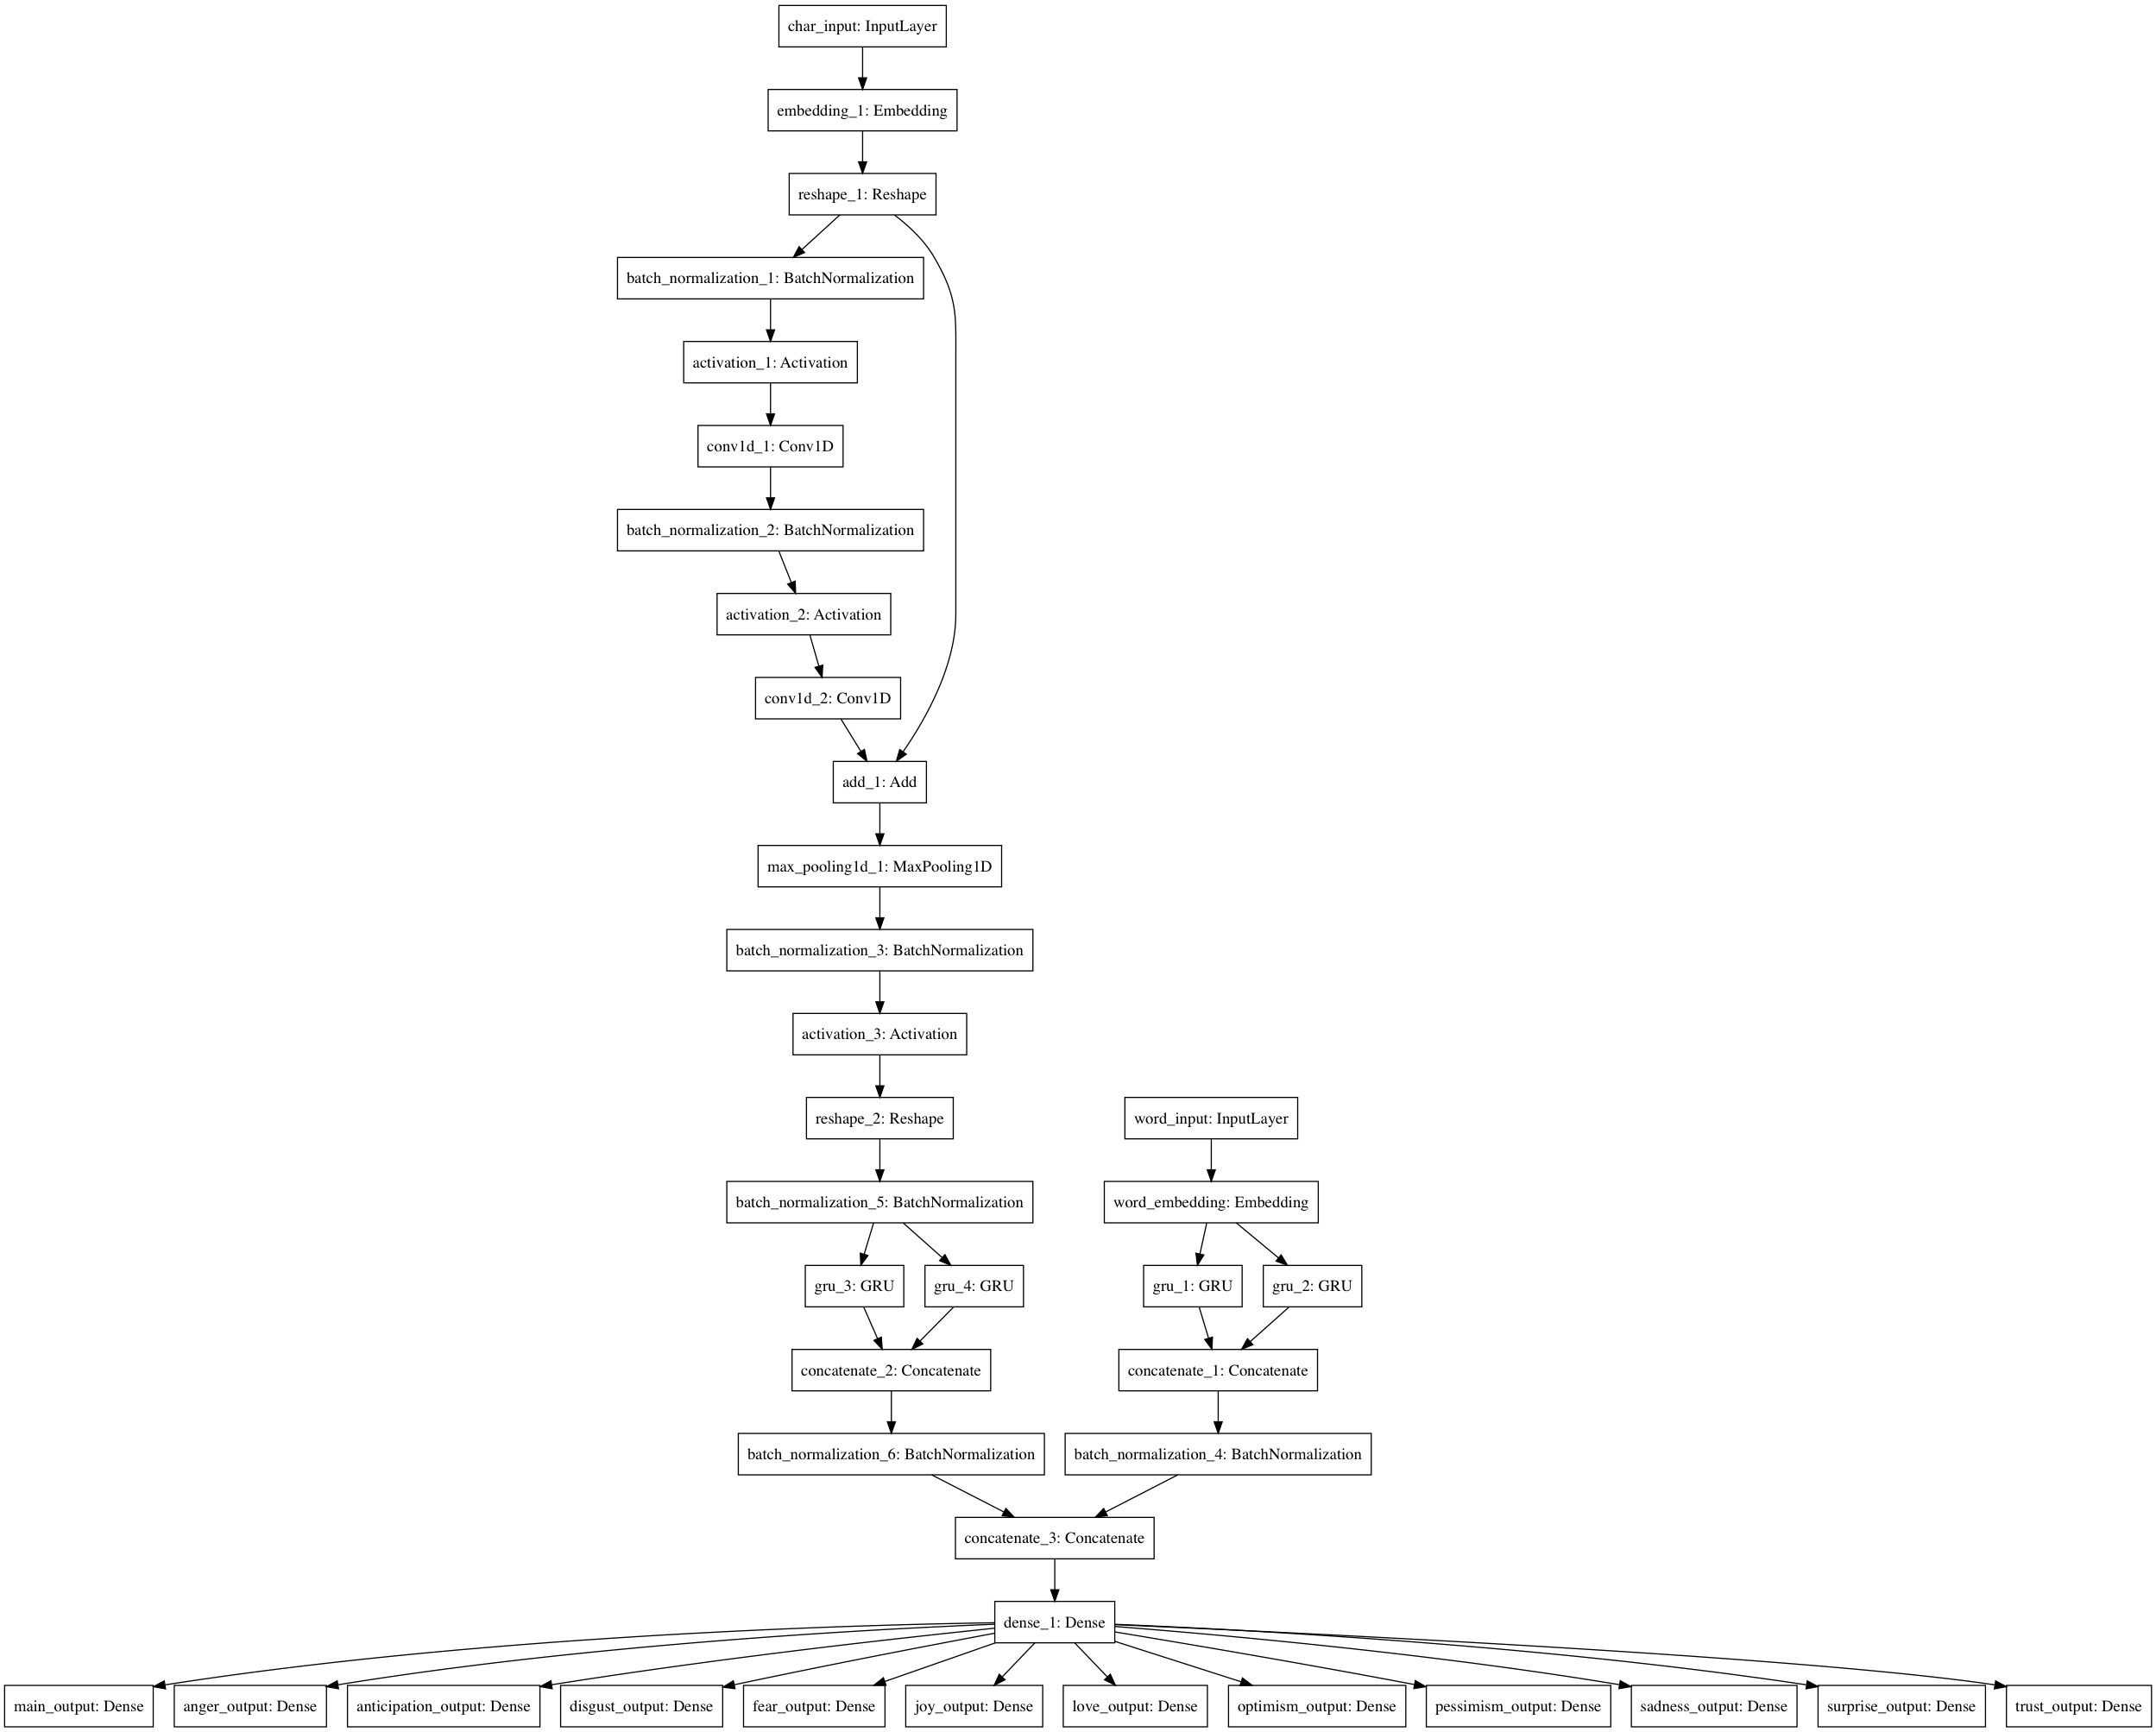
\includegraphics[width=\textwidth]{pictures/model.png}
        \caption{The full model, training on both word and character representations}
        \label{fig:fullmodel}
\end{figure}

\subsection{Model output}
Since the model reads in all regression data in one single input and outputs it in a similar bulk manner, the overall feeling from the regression data can not be intrinsically inferred from the regression value, meaning, the way that an "anger tweet" is classified as an anger tweet is its position in the large output matrix. That way, if a completely new tweet would be presented to the model, the value of the regression would be an emotion intensity felt by the tweeter but in a general sense. To help guide the intensity in a direction, the eleven classification labels could be used to infer the tweeters general state of mind. 

\subsection{Loss functions}
Since the model is a multitask model, more than one loss function was needed. The model solves two tasks which can not share loss functions, because of the inherent nature of the problem. One is a regression problem and the other a classification.

\subsubsection{Regression loss function and metric}
For the regression output of the model, mean squared error was chosen as a way to optimize the model with regards to Pearson-score \ref{eq:pearson}. Mean squared error is used in the following form:\\
\begin{equation} \label{eq:lreg}
L_{reg}(gold, pred)=\dfrac{1}{b_{size}}\sum^{b_{size}}_{i=1}\left(gold_{i}-pred_{i}\right)^{2}
\end{equation}\\
The metric used for the regression is mean absolute error:\\
\begin{equation} \label{eq:meanabs}
m_{reg}=\dfrac{1}{b_{size}}\sum^{b_{size}}_{i=1}abs\left(gold_{i}-pred_{i}\right)
\end{equation}\\
Where $b_{size}$ is the batch size used by the model during training. 

\subsubsection{Classification loss function and metric}
The loss function for the classification is a bit more convoluted since all regression tweets have regression labels but not all regression tweets have classification labels. This is handled by way of a mask and the augmentation specified in section \ref{sec:augm}. The loss function is described as such:\\
\begin{equation} \label{eq:fclass}
f(gold,pred) =
     \begin{cases}
       0, &\quad\text{if gold = mask}\\
       wbce(gold,pred), &\quad\text{otherwise} \\
     \end{cases}
\end{equation}\\
where \textit{wbce} is our custom weighted binary cross entropy function. Since the model has eleven output layers, there is a loss function for each of the eleven emotions/layers. The function (\ref{eq:fclass}) is used in a batch wise manner as in the regression case on each emotion:\\
\begin{equation} \label{eq:lemotion}
L_{emotion}=\dfrac{1}{b_{size}} \sum_{i=1}^{b_{size}} f(gold_i, pred_i)
\end{equation}\\
 This loss function ensures that tweets with no classification labels do not impact the updating of the weights of the model by giving the predicted values a loss of zero.\\
Binary cross entropy is defined as follows:\\
\begin{equation}
BCE(gold,pred) = -(gold \cdot log(pred)+(1-gold) \cdot log(1-pred))
\end{equation}\\
The custom weighted binary cross entropy function is defined as follows:\\
\begin{equation} \label{eq:wBCE}
wBCE(gold,pred) = (gold \cdot 1_{weight} + (1-gold) \cdot 0_{weight}) \cdot BCE(gold, pred)
\end{equation}\\
where $1_{weight}$ and $0_{weight}$ are parameters that can be tuned in the model. This weighting parameter is included because of the uneven distribution of ones and zeros. The goal of the model is to detect whenever emotions are felt by the tweeter, and as such ones are to be valued more if guessed.  \\ \\
The metric used for classification is a custom metric function which builds on binary accuracy. The custom part consists of masking the -1's the same way as the loss function, so that the metric returns a value corresponding to a correct guess whenever classification labels are missing. The custom metric function looks like this: \\
\begin{equation}
f(gold,pred) =
     \begin{cases}
       1, &\quad\text{if gold = mask}\\
       BA(gold,pred), &\quad\text{otherwise} \\
     \end{cases}
\end{equation}\\
where \textit{BA} is defined as follows: \\
\begin{equation} \label{eq:bin_acc}
BA(gold, pred) =
	\begin{cases}
		1, &\quad\text{if gold = round(pred)} \\
		0 &\quad\text{otherwise} \\
	\end{cases}
\end{equation}\\
where the \textit{pred} value is rounded to 0 or 1 since it is a probability value of the guessed emotion.\\
This equation is then used and averaged batch-wise like the loss: \\
\begin{equation} \label{eq:class_metric}
m_{class}=\dfrac{1}{b_{size}}\sum^{b_{size}}_{i=1}f\left(gold_{i}-pred_{i}\right)
\end{equation}\\

\subsubsection{Combined loss function}
The model is trained using the sum of equation (\ref{eq:lreg}) and (\ref{eq:lemotion}):\\
\begin{equation} \label{eq:lratio}
L_{combined}(gold,pred)=L_{ratio}\cdot L_{reg}(gold, pred) +  \sum_{e\in E}\dfrac{(1-L_{ratio})}{|E|}\cdot L_{e}(gold, pred),
\end{equation}\\
where \textit{e} is one of the eleven emotions in \textit{E}. The ratio $L_{ratio}$ is a parameter that can be tweaked and can be used to force the model implicitly to weight one task higher than the other. Furthermore, the weighting of the single classification emotions can also be tweaked and given more weighting than the others.

\subsection{Hyperparameter testing}
\subsubsection{Regression, task 1}
In figure \ref{fig:averagedropout} the Pearson score is plotted with regards to the different dropout values.
\begin{figure}[H]
    \centering
        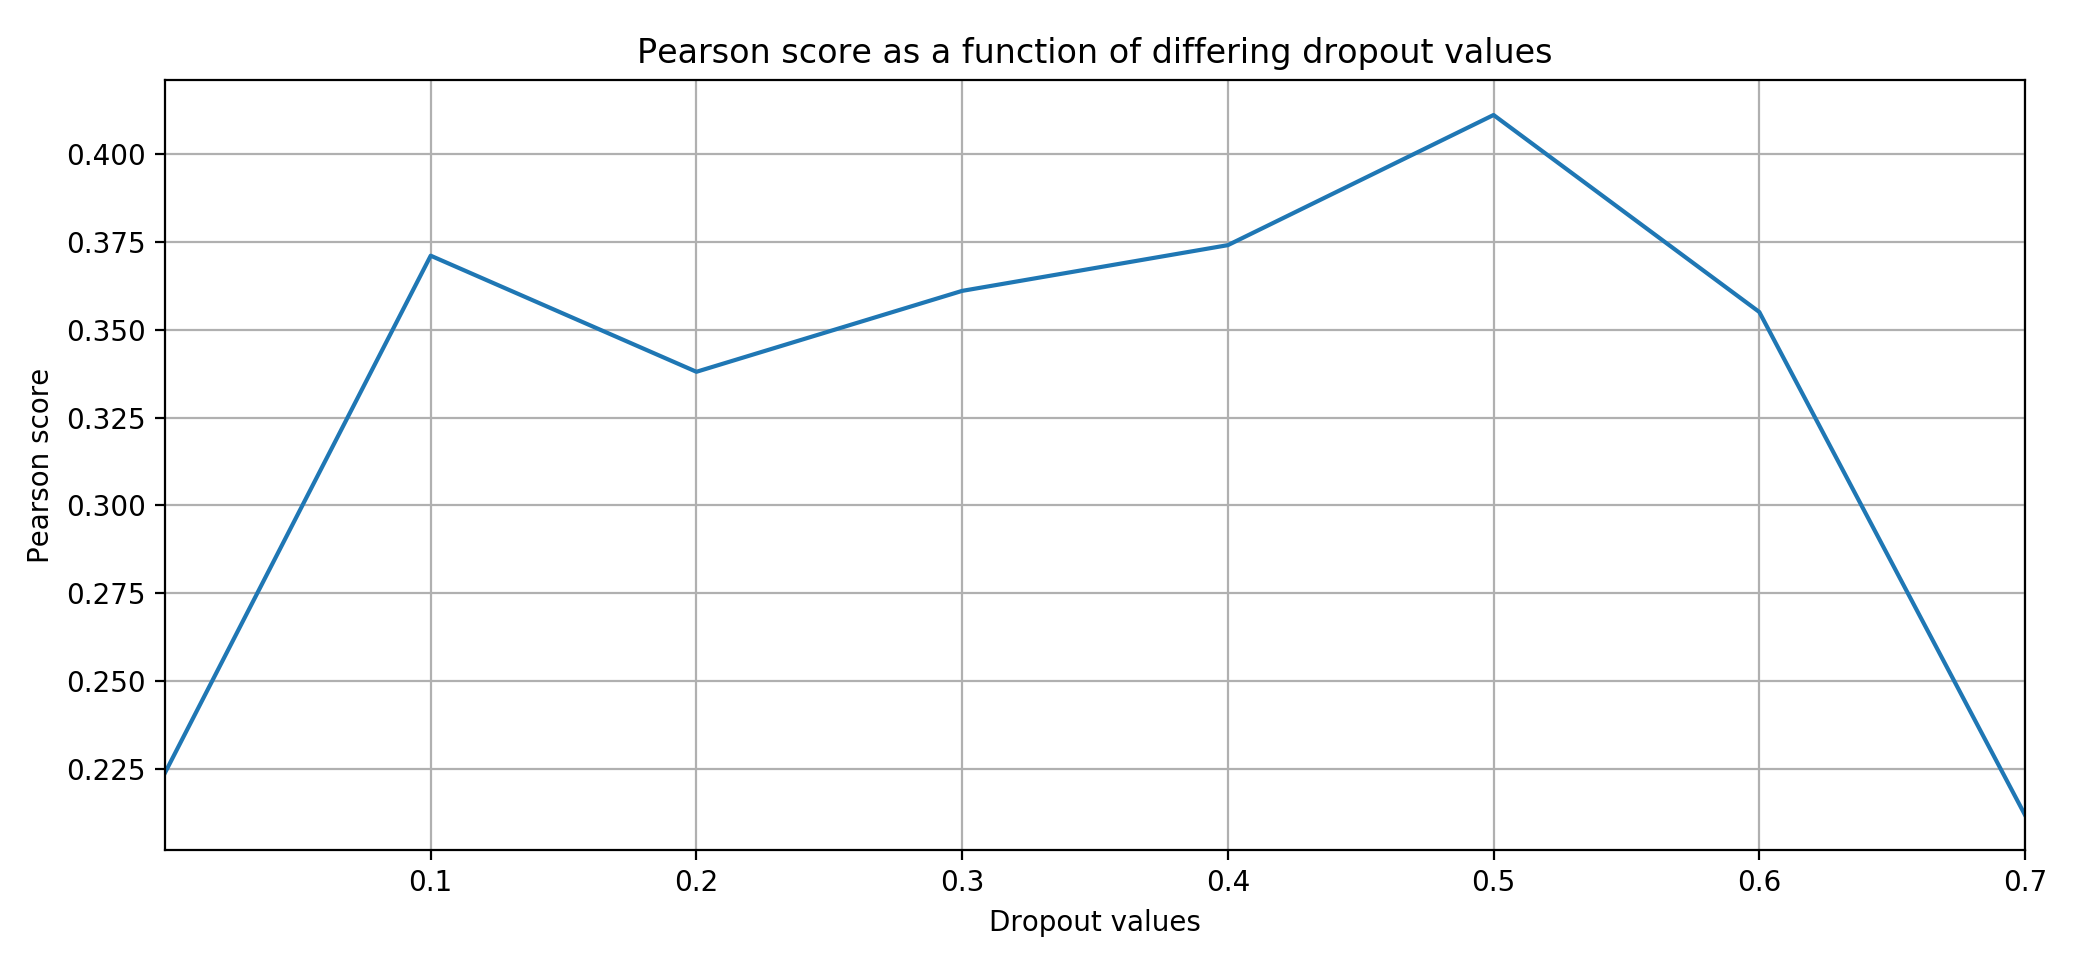
\includegraphics[width=\textwidth]{pictures/DropoutPlot.png}
        \caption{Pearson scores as a function of dropout value, loss weight set to 0.45, weighted BCE set to 0.5}
        \label{fig:averagedropout}
\end{figure}
It is evident that dropout values higher than 0.5 results in worse Pearson scores. This is because of the models tendency to underfit because of the sheer amount of hidden units getting dropped in every run. Furthermore, predictions on joy is significantly worse than the other regression emotions.\\
\\
The weighting in the binary cross entropy, as used in equation (\ref{eq:wBCE}) still has an interplay with the Pearson score reached by the model, since the two tasks are solved jointly, as thus this correlation is relevant.
\begin{figure}[H]
    \centering
        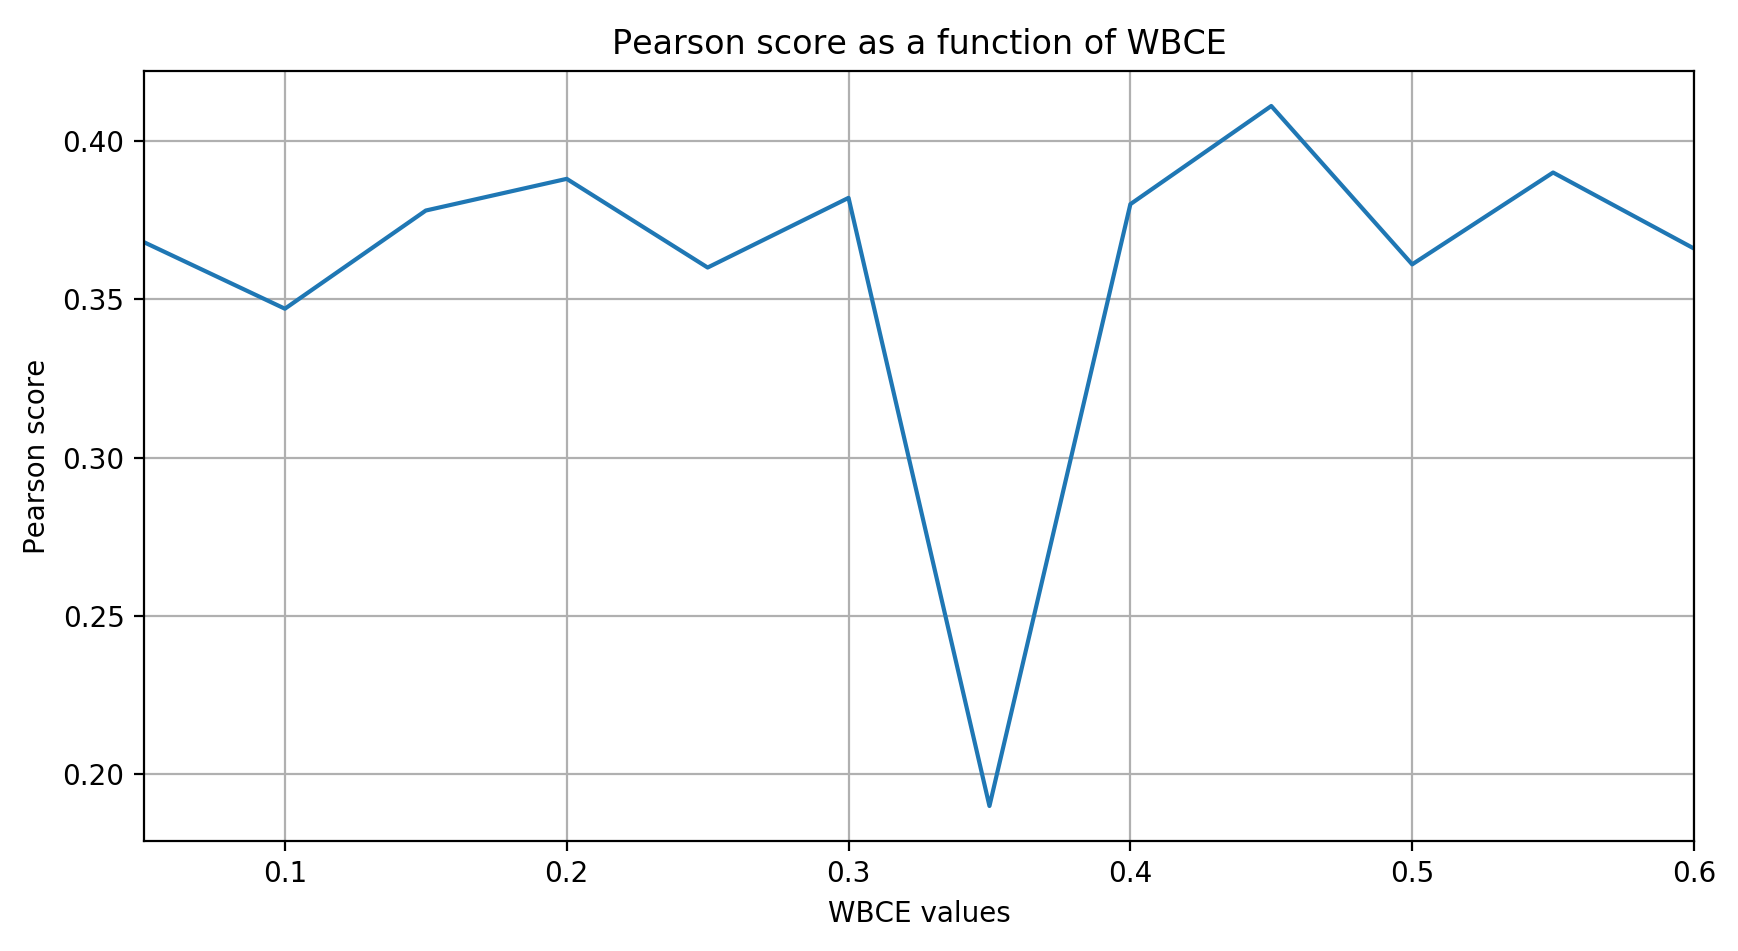
\includegraphics[width=\textwidth]{pictures/weightedBCEplot.png}
        \caption{Average Pearson score as a function of weighted BCE value, dropout set to 0.3, loss weight set to 0.45}
        \label{fig:averageBCE}
\end{figure}
The weightings shown in figure \ref{fig:averageBCE} is the weight of the zeros and the one weights are then $1-0_{weight}$, as outlined in equation (\ref{eq:wBCE}).\\
In figure \ref{fig:averageBCE} it can be seen that the effect of the weighting is not wholly insignificant. The best Pearson score is reached with a weighting of zeros to 0.45 and ones to 0.55. Beyond a weight of 0.6, that is, weighting zeros 0.6 and ones 0.4 the Pearson score started dropping off. It is unclear why the outlier at a weighting of 0.35 deviates so much from the general tendency, since the model and predictions were healthy, albeit very bad.\\
\\
The loss weights plotted in figure \ref{fig:averageLW} are the loss weights as outlined in equation (\ref{eq:lratio}).
\begin{figure}[H]
    \centering
        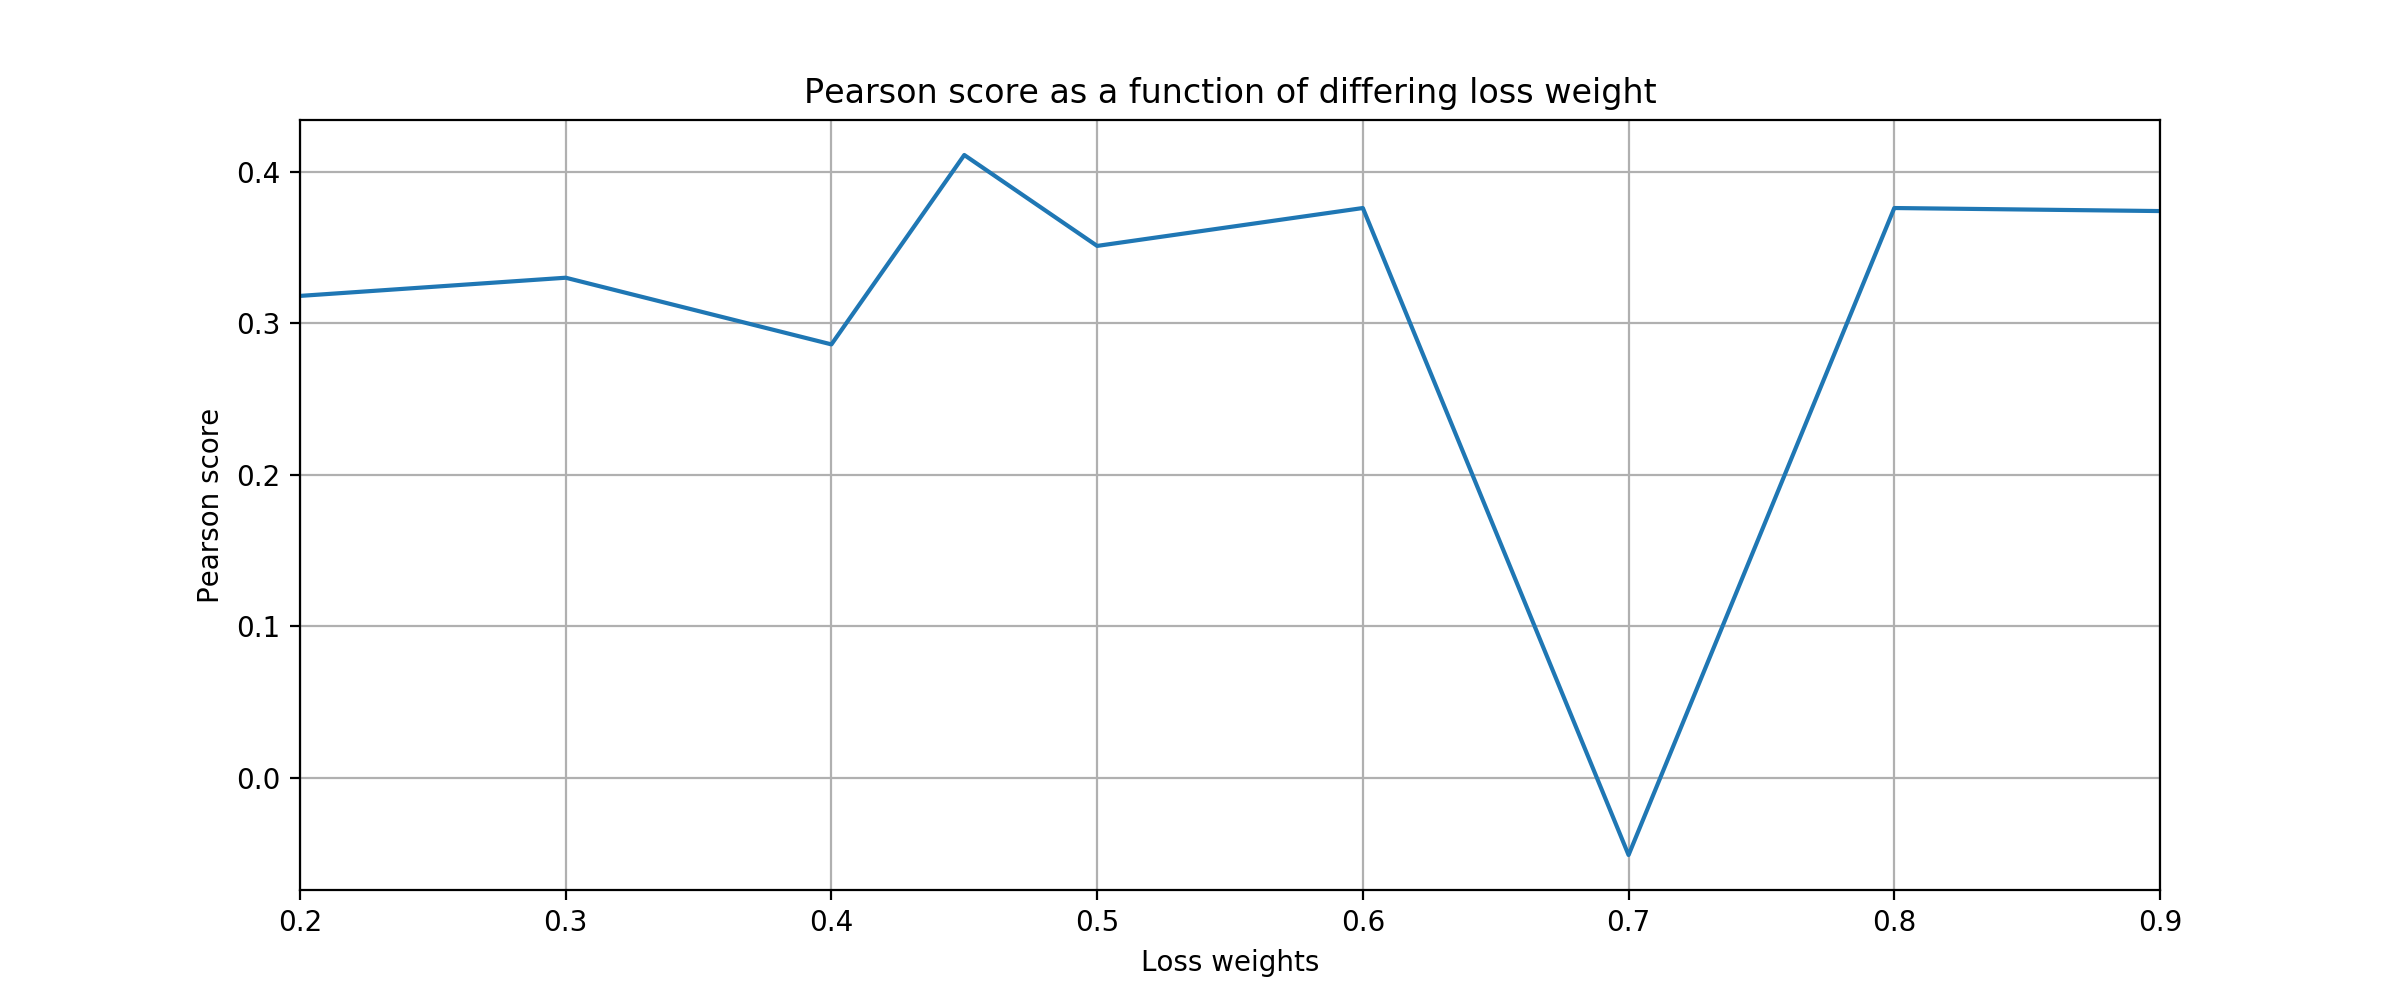
\includegraphics[width=\textwidth]{pictures/LossWeightsPlot.png}
        \caption{Average Pearson scores as a function of loss weight value, dropout set to 0.3, weighted BCE set to 0.45}
        \label{fig:averageLW}
\end{figure}
The loss weights have an outlier, and much like the outlier in the testing of weights for the binary cross entropy, is it unclear why it is present as the model guessed in the correct form, just badly.\\
The general tendency of the loss weights was not fully as to be expected, meaning, a high weighting towards the regression task would yield a better Pearson score. This might have to do with the fact that the embedding weights being trained to do minimize the weighted sum of the two loss function (equation (\ref{eq:lratio})) might not favor one task heavily over the other, i.e. the two tasks have an overlap in the weights that solve them and in the overall structure of the tasks.

\begin{table}[h]
\centering
\begin{tabular}{c|c|c|c|c|c|}
& \text{Anger} & \text{Fear} & \text{Joy} & \text{Sadness} & \text{Avg.} \\ \hline
\text{No embedding} & 0.249 & 0.471 & 0.208 & 0.362 & 0.323 \\
\text{Embedding} & 0.382 & 0.520 & 0.108 & 0.434 & 0.361
\end{tabular}
\caption{Pearson scores with and without pre-trained word embeddings}
\label{tab:no_emb}
\end{table}

From table \ref{tab:no_emb}, it is clear that embeddings give  a better score than no embeddings, although one noticeable difference is the Pearson score for joy. This could have something to do with the pretrained embedding weights not having a good instantiation towards the more positively weighted words, which then skews the results for that particular emotion.  

\begin{table}[h]
\centering
\begin{tabular}{c|c|c|c|c|c|}
& \text{Anger} & \text{Fear} & \text{Joy} & \text{Sadness} & \text{Avg.} \\ \hline
\text{NADAM} & 0.282 & 0.480 & 0.205 & 0.373 & 0.335 \\
\text{ADAM} & 0.405 & 0.457 & 0.150 & 0.429 & 0.360
\end{tabular}
\caption{Pearson scores with NADAM and ADAM optimizers}\label{tab:NADAM_ADAM}
\end{table}

Some light testing was done in way of optimizers used for the model. The final choice of optimizer was the ADAM optimizer with a learning rate of 0.001, a learning rate decay of $10^{-5}$ and clipping the gradients to 1. The only difference between the two optimizers was that NADAM used Nesterov momentum. Explaining the difference and going in-depth with optimizers is beyond the scope of this report, and only superficial tests were done between the two. \\
\\
More detailed barplots of the different runs can be seen in the appendix, figures \ref{fig:dropoutvalues}, \ref{fig:BCEvalues} and \ref{fig:LWvalues}.
\subsubsection{Classification, task 5}
In figure \ref{fig:dropoutacc} the accuracy is plotted with regards to the dropout values.
\begin{figure}[H]
    \centering
        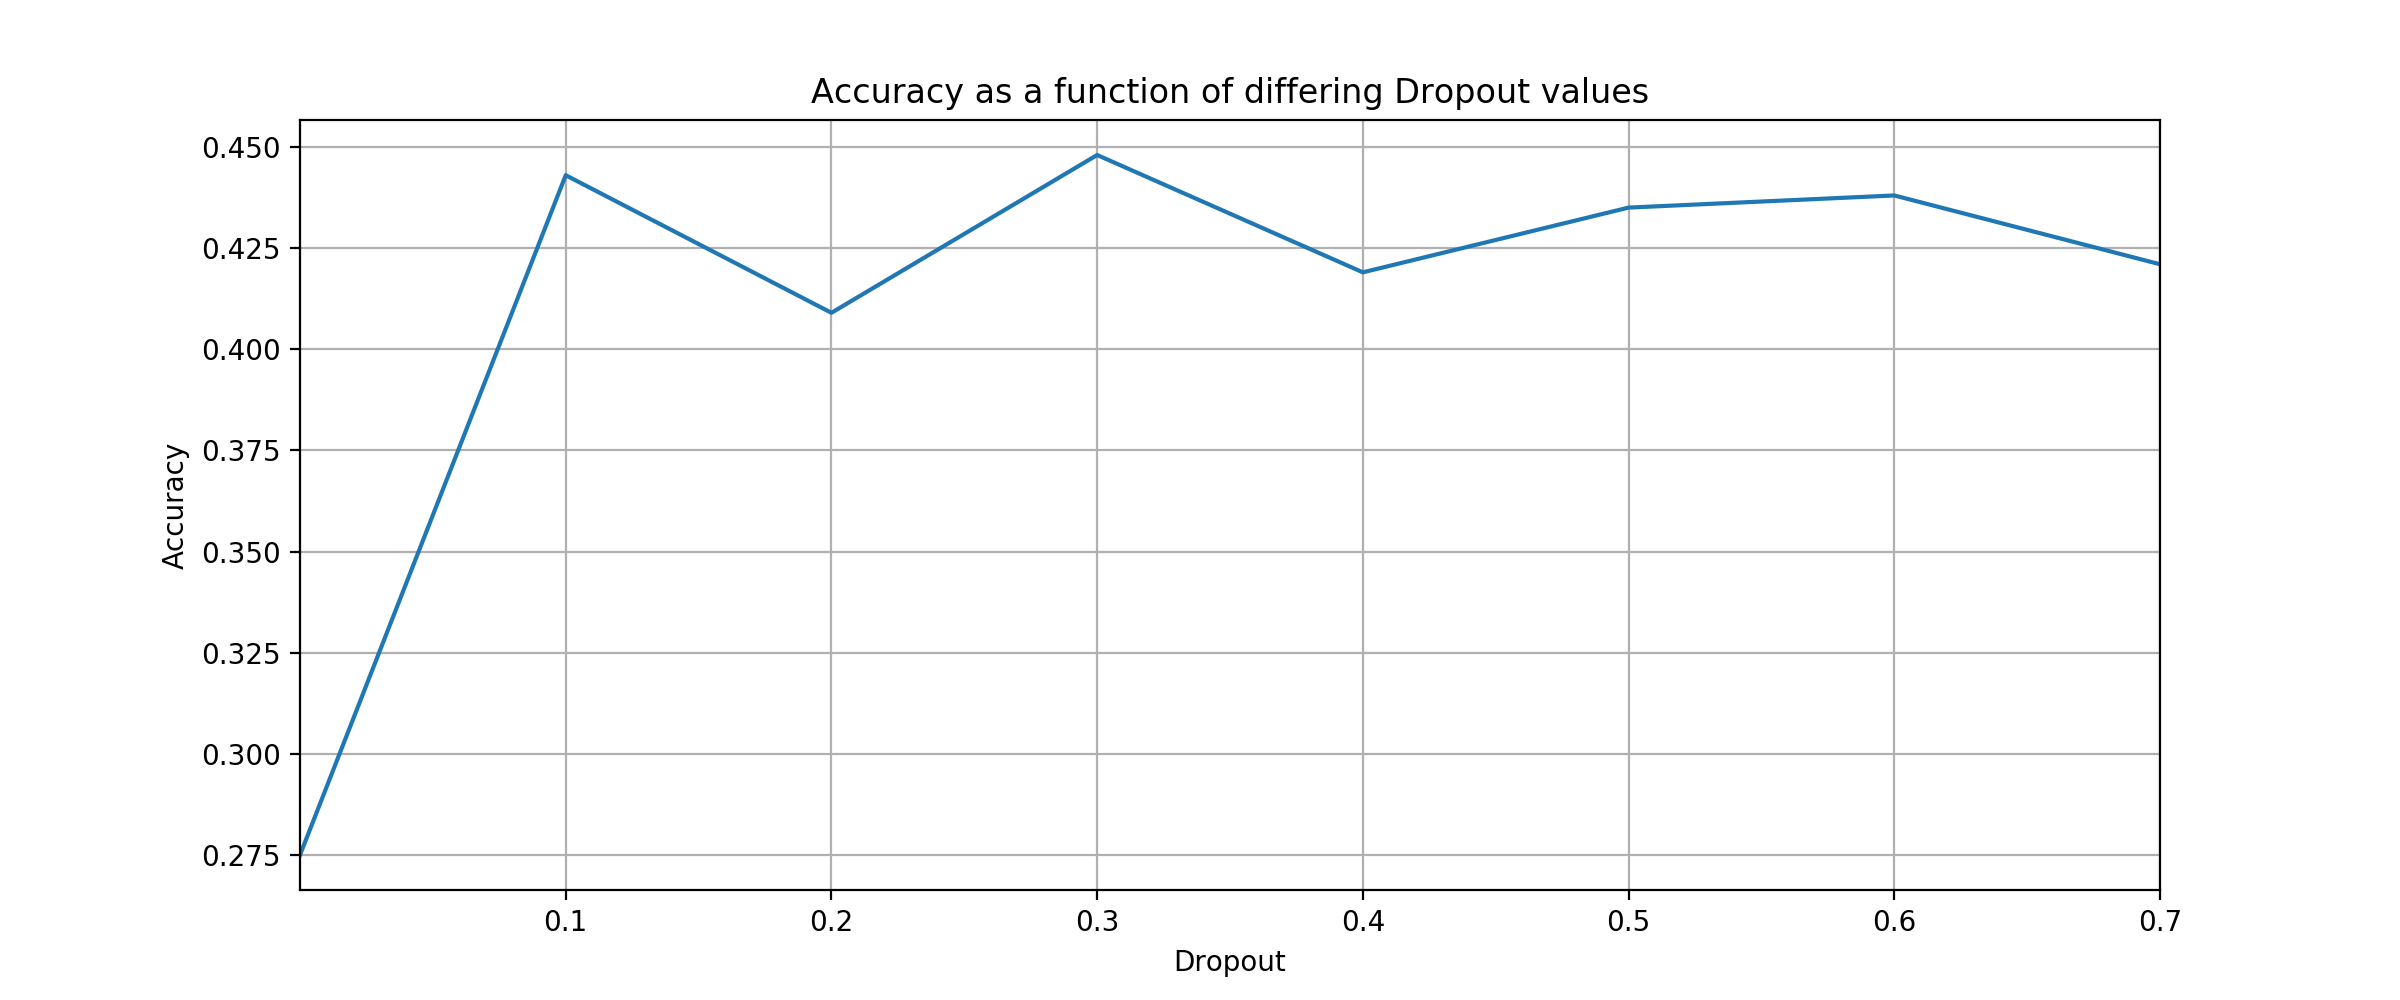
\includegraphics[width=\textwidth]{pictures/DropoutPlotAcc.png}
        \caption{Accuracy as a function of dropout value, loss weight set to 0.45, weighted BCE to 0.45}
        \label{fig:dropoutacc}
\end{figure}
As seen in the regression case, some dropout is needed, but there is not a clear tendency whether or not a specific dropout value is significantly better than the others.\\
\\
In figure \ref{fig:bceacc} the accuracy is plotted with regards to the different weighted BCE values.
\begin{figure}[H]
    \centering
        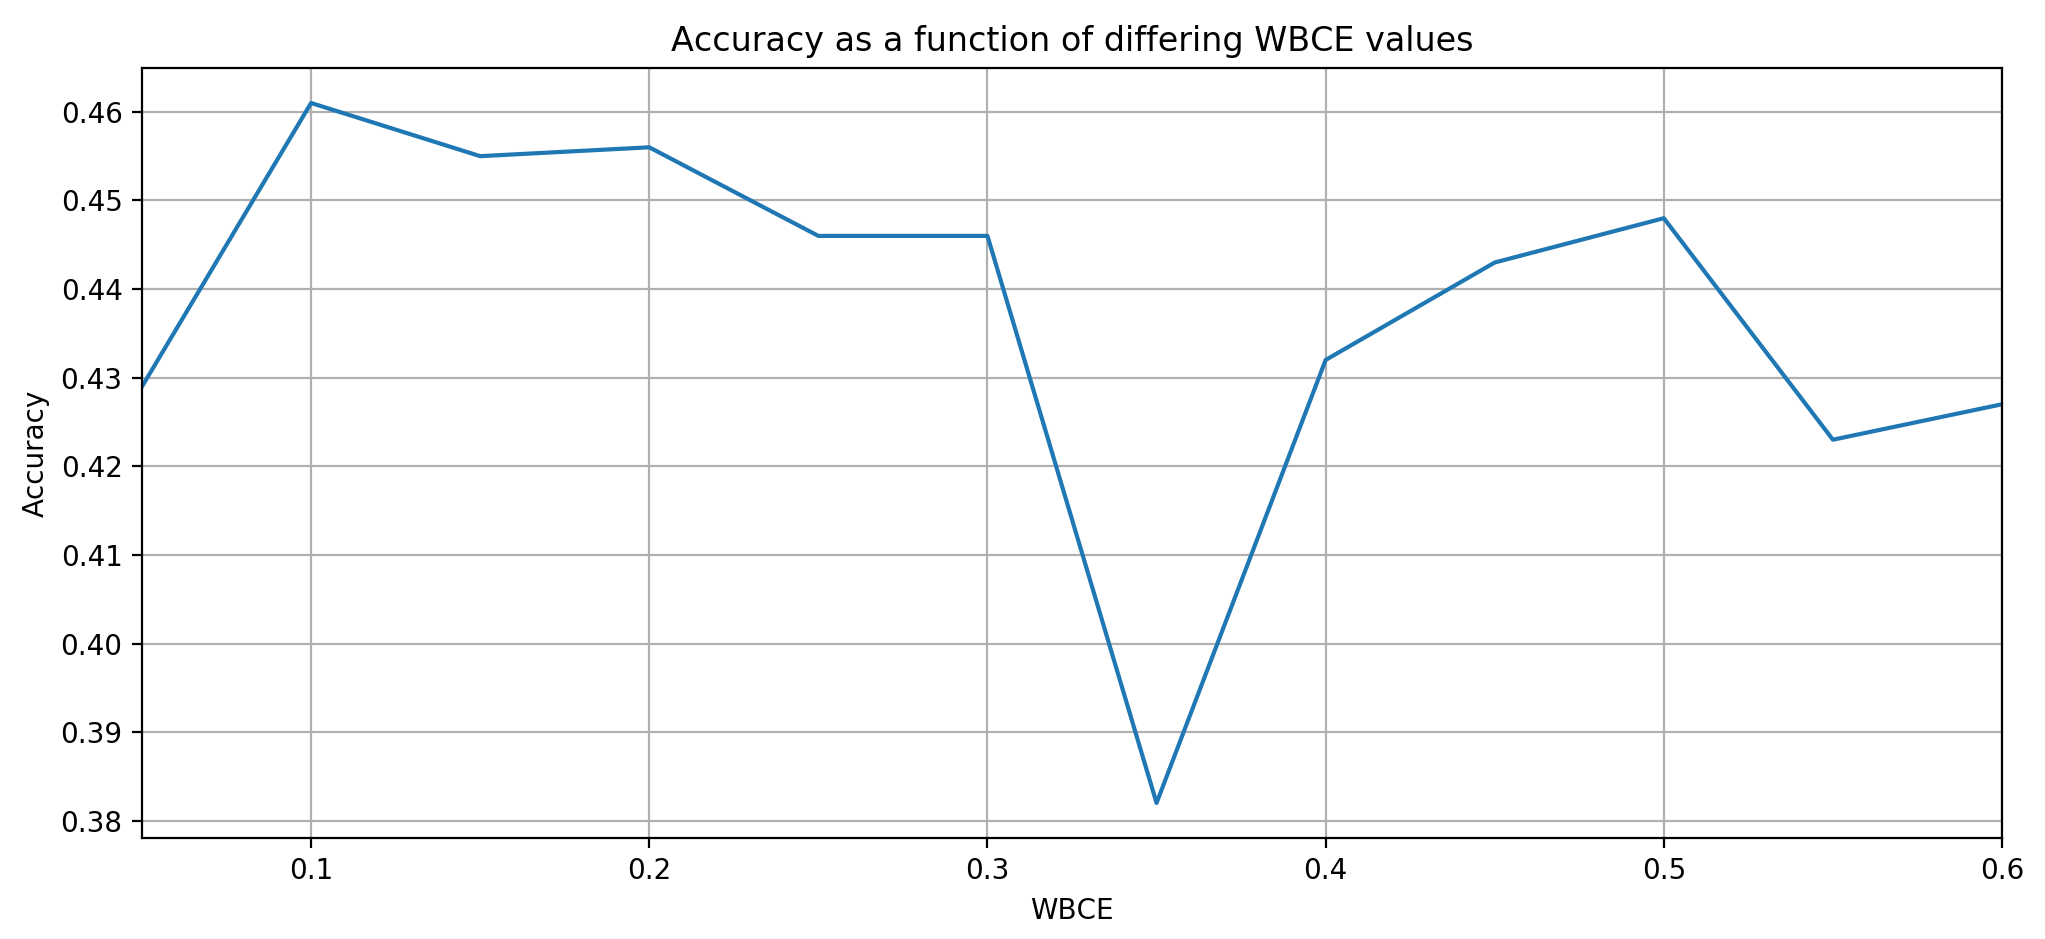
\includegraphics[width=\textwidth]{pictures/WBCEPlotAcc.png}
        \caption{Accuracy as a function of weighted BCE value, loss weight set to 0.45, dropout set to 0.3}
        \label{fig:bceacc}
\end{figure}
As can be seen in figure \ref{fig:bceacc}, there is an outlier at a weighted BCE value of 0.35. It is also noticeable that at a weighted BCE value of 0.1, meaning that a weighting of zeros to a tenth of the summed loss contribution, the accuracy gets noticeably better. This value was not chosen, however, as it drastically reduced the Pearson score of the model, as seen in figure \ref{fig:averageBCE}, the overall loss would then be worse. \\
\\
In figure \ref{fig:lwacc} the accuracy is plotted with regards to the different loss weight values. 
\begin{figure}[H]
    \centering
        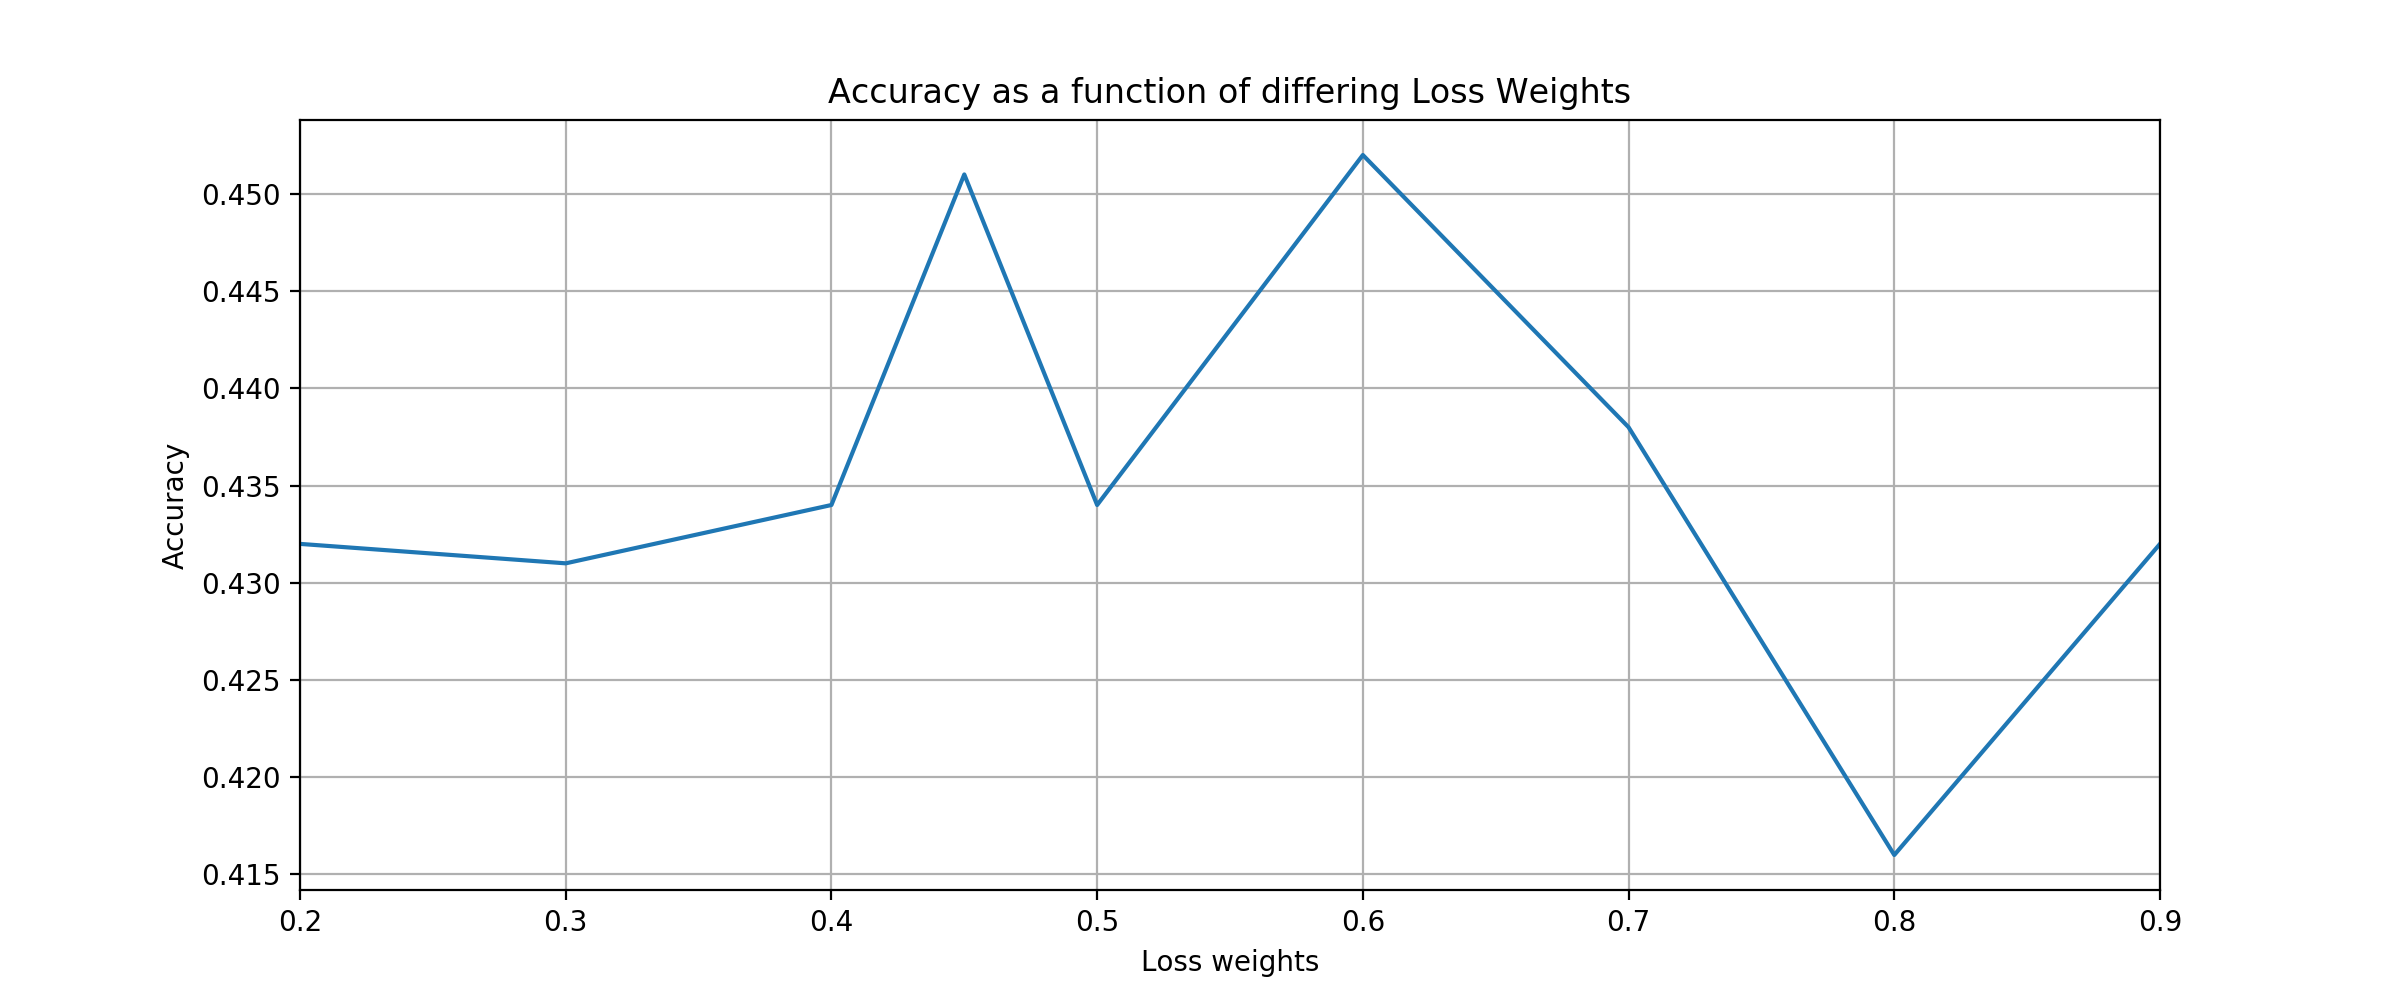
\includegraphics[width=\textwidth]{pictures/LossWeightPlotAcc.png}
        \caption{Accuracy as a function of loss weight value, weighted BCE set to 0.45, dropout set to 0.3}
        \label{fig:lwacc}
\end{figure}
As with the regression case, the Pearson score at the different loss weights would be expected to have a larger impact.

\subsection{Results and data}
The final model used was zeroed in on through an experimental basis. It used $0_{weight}=0.45$ and $1_{weight}=0.55$, a dropout of 0.5 and $L_{reg}=0.45$ and $L_{class}=0.55$. 400 dimensional word and char embeddings and a 250 dimensional GRU was used for each submodel. The resulting sanity check yielded following results:
\begin{table}[H]
\centering
\begin{tabular}{c|c|c|c|c}
\text{Anger} & \text{Fear} & \text{Joy} & \text{Sadness} & \text{Avg.} \\ \hline
0.865 & 0.896 & 0.882 & 0.897 & 0.885 \\
\end{tabular}
\caption{Sanity check Pearson scores for regression}
\label{tab:sanityreg}
\end{table}

\begin{table}[H]
\centering
\scalebox{0.7}{\begin{tabular}{c|c|c|c|c|c|c|c|c|c|c|c|c}
\multicolumn{12}{c}{\textbf{F-micro}} & \textbf{Global accuracy}\\ \hline
Anger & Anticipation & Disgust & Fear & Joy & Love & Optimism & Pessimism & Sadness & Surprise & Trust & Neutral & \\ \cline{1-12}
0.968 & 0.931 & 0.964 & 0.971 & 0.982 & 0.931 & 0.955 & 0.899 & 0.951 & 0.909 & 0.905 & 0.833 & 0.933 \\
\end{tabular}}
\caption{Sanity check scores for classification}
\label{tab:sanityclass}
\end{table}
The results of the final model on the development data is shown in tables \ref{tab:devreg} and \ref{tab:devclass}.

\begin{table}[H]
\centering
\begin{tabular}{c|c|c|c|c}
\text{Anger} & \text{Fear} & \text{Joy} & \text{Sadness} & \text{Avg.} \\ \hline
0.371 & 0.555 & 0.184 & 0.532 & 0.411 \\
\end{tabular}
\caption{Pearson scores for regression on development data}
\label{tab:devreg}
\end{table}

\begin{table}[H]
\centering
\scalebox{0.7}{\begin{tabular}{c|c|c|c|c|c|c|c|c|c|c|c|c}
\multicolumn{12}{c}{\textbf{F-micro}} & \textbf{Global accuracy}\\ \hline
Anger & Anticipation & Disgust & Fear & Joy & Love & Optimism & Pessimism & Sadness & Surprise & Trust & Neutral & \\ \cline{1-12}
0.687 & 0.232 & 0.626 & 0.638 & 0.685 & 0.416 & 0.574 & 0.179 & 0.555 & 0.141 & 0.038 & 0.053 & 0.443 \\
\end{tabular}}
\caption{Classification scores on development data}
\label{tab:devclass}
\end{table}
